\documentclass[border=4pt]{standalone}
\usepackage[T1]{fontenc}
\usepackage{helvet}
\renewcommand{\familydefault}{\sfdefault}
\usepackage{graphicx}
\usepackage{caption}
\usepackage{amsmath}
\captionsetup{font={sf,footnotesize},labelfont={sf,bf,footnotesize},justification=justified,singlelinecheck=false}
\begin{document}
\setcounter{figure}{1}
\begin{minipage}{7.20in}
\centering
\begin{figure}[htbp]
    \centering
    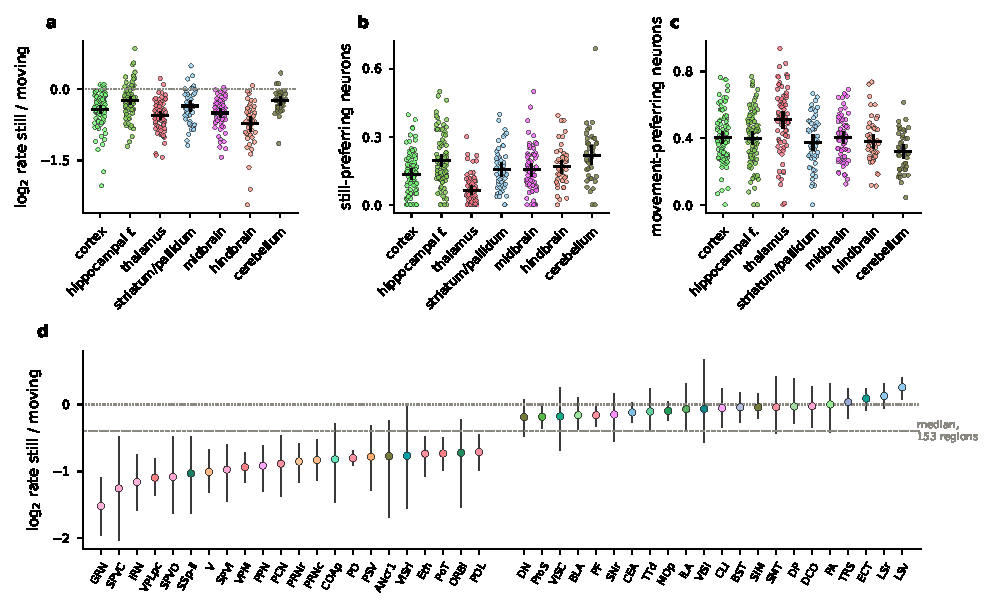
\includegraphics[width=\linewidth]{fig2_rates_panels.pdf}
    \caption{Stillness lowers firing across the brain; orofacial brainstem and thalamus are suppressed most, hippocampus and cerebellum least. \textbf{a} Population firing in awake stillness relative to movement, log$_2$ of the rate ratio, one dot per mouse (neurons averaged within mouse and division, mice with $\geq$5 neurons); black: mean over mice and 95\% bootstrap CI. Over all neurons 99\% of 130 mice are below zero. \textbf{b} Fraction of still-preferring neurons (0.5\,s epoch Welch test, $p<0.01$, higher in stillness). \textbf{c} Fraction of movement-preferring neurons. \textbf{d} The 22 regions with the strongest and the 22 with the weakest suppression in stillness, among the 153 regions recorded in $\geq$5 mice (mean over mice, mouse-bootstrap 95\% CI; dots in Allen atlas region colours; * conservative DMN core).}
    \label{fig:rates}
\end{figure}
\end{minipage}
\end{document}
